\section[组合编码和伪距观测]{组合编码和伪距观测\\Combined Code and Phase Observations}

GPS观测值的特点是在短时间间隔内收集大量数据,时间间隔由1s到30s变化不等。在实时定位或者后处理模式中,利用最小二乘或者本章描述的滤波进行数据处理。获取高精度的计算方法需要更长时间的观测数据,而其他的定位计算方法着重于短时间数据处理或者实时可用性。

当前最好的大地接收机可以传送双频P码和相位观测值,我们应该限制使用静态天线处理观测数据的最新方法。数据后处理可以达到最高的精度。

处理GPS观测数据最常用的方法是使用双差观测值。这种双差观测值对于两台接收机位置的相同误差是不敏感的,而一台接收机相对于另一台接收机的变化值却是非常敏感的。因此,双差观测值类似于传统的距离与方向观测值。

为了从整周模糊度中分离几何向量(即两台接收机间的基线),我们需要更多的数据。在没有先验信息情况下,很难在短时间内从模糊度中求出基线向量。但是随着时间的推移,有一条基线符合双差观测是有希望的。观测的卫星数越多,基线向量就越快被确定下来。只要基线在一周的小数部分中唯一确定,那么就可以确定整周模糊度。这是最佳使用双差观测的关键。

通常利用最小二乘原理估计模糊度和基线向量,即残差的平方和最小。模糊度常被看做实数,因为随着系统误差的确定,模糊度逐渐趋向整数值。模糊度能够被准确固定的短基线案例被视为经典案例。

\begin{figure}
	\centering
	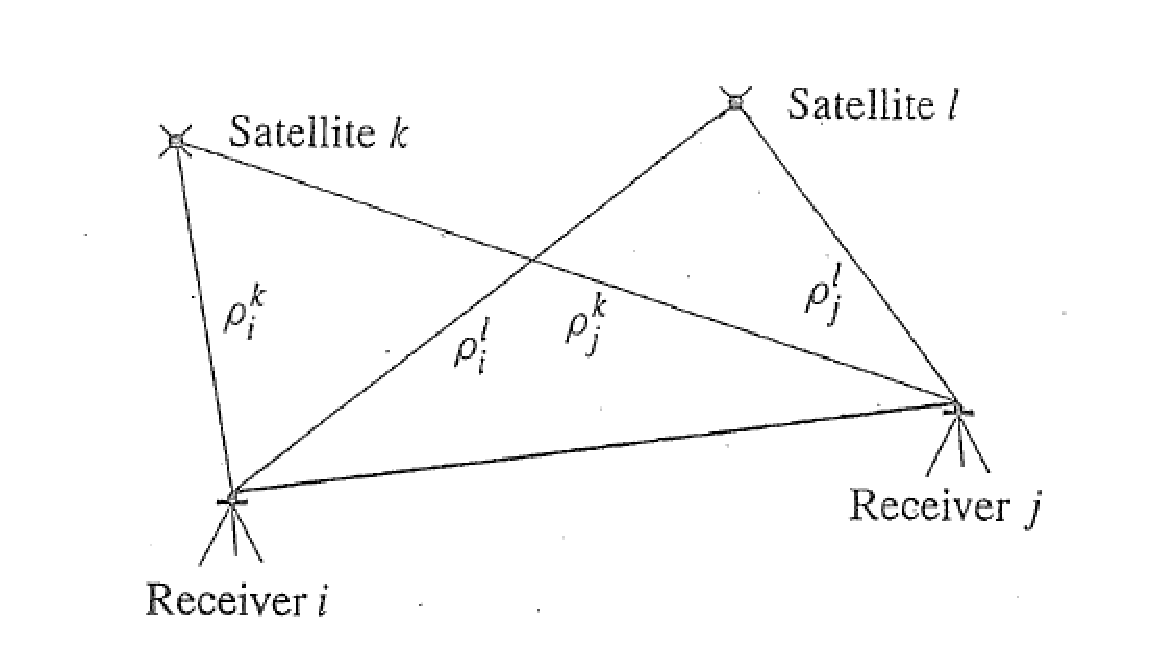
\includegraphics[width=0.4\linewidth]{TeX_files/Part03/chapter10/image/9-2}
	\caption{双差$\rho_{i}^{k}-\rho_{i}^{l}-\rho_{j}^{k}+\rho_{j}^{l}$,两台接收机同步观测到两颗卫星的伪距}
	\label{fig:9-2}
\end{figure}

我们应该使用Yang 、Goad和Schaffrin(1994)介绍的术语以供参考。理想的伪距$\rho^{*}$是独立于时钟项的所有频率的组合值:
\begin{equation}
	\rho_{i}^{*k}=\rho_{i}^{k}(t,t-\tau_{i}^{k})+T_{i}^{k}+c(dt_{i}(t)-dt^{k}(t-\tau_{i}^{k}))
\end{equation}

如果电离层的影响$I_{i}^{k}$为零,则$\rho^{*}$与伪距$\rho$是相同的。项$T_{i}^{k}$表示对流层延迟。当我们使用双差观测值时,括弧里的项就消除了,因为它们都是钟差项。

相位观测值$\Phi_{i}^{k}(t)$是在同一频率下产生的信号相位差作为伪距,基础方程为:
\begin{equation}
	\Phi_{i}^{k}(t)=\rho_{i}^{k}-I_{i}^{k}+T_{i}^{k}+c(dt_{i}(t)-dt^{k}(t-\tau_{i}^{k}))+\lambda(\varphi_{i}(t_{0})-\varphi^{k}(t_{0}))+\lambda N_{i}^{k}-\epsilon_{i}^{k}
\end{equation}

新增项是卫星k和接收机i之间的模糊度$N_{i}^{k}$、以及非零初始相位$\varphi^{k}(t_{0})$和$\varphi_{i}(t_{0})$。再次介绍上面给出的理想伪距:
\begin{equation}
	\Phi_{i}^{k}(t)=\rho_{i}^{*k}+\lambda N_{i}^{*k}
\end{equation}

此处$N_{i}^{*k}=N_{i}^{k}+\varphi_{i}(t_{0})-\varphi^{k}(t_{0})$。 双差观测中,两个$\varphi$项和两个dt项都被消除。此时,双差观测中$N_{ij}^{*kl}=N_{ij}^{kl}$,这将在接下来的(10.6)和(10.7)得到应用。

下面详细演示了如何对观测值做双差。原始观测值是一台接收机与一颗卫星之间的距离差(单程),两台接收机对同一颗卫星做差可以估计卫星钟差;最后两台接收机对两颗卫星做差可以估计接收机钟差。接收机为i和j,卫星为k和l:
\begin{equation}
	On L1: P_{1,ij}^{kl}=\rho_{i}^{k}-\rho_{i}^{l}-\rho_{j}^{k}+\rho_{j}^{l}+I_{ij}^{kl}+T_{ij}^{kl}-e_{1,ij}^{kl}
\end{equation}

\begin{equation}
	On L2: P_{2,ij}^{kl}=\rho_{i}^{k}-\rho_{i}^{l}-\rho_{j}^{k}+\rho_{j}^{l}+(f_{1}/f_{2})^{2}I_{ij}^{kl}+T_{ij}^{kl}-e_{2,ij}^{kl}
\end{equation}

很明显$T_{ij}^{kl}=(T_{i}^{k}-T_{i}^{l})-(T_{j}^{k}-T_{j}^{l})$,同样的$I_{ij}^{kl}$、 $N_{ij}^{kl}$ 和$\epsilon_{ij}^{kl}$。L1和L2 载波信号的下标1和2分别对应着频率$f_{1}$和$f_{2}$。 为了强调卫星几何分布的影响,$\rho$项不进行组合,他们仍然是双差,因此相位观测方程为:
\begin{equation}
	\Phi_{1,ij}^{kl}=\rho_{i}^{k}-\rho_{i}^{l}-\rho_{j}^{k}+\rho_{j}^{l}-I_{ij}^{kl}+T_{ij}^{kl}+\lambda_{1} N_{1,ij}^{kl}-\epsilon_{1,ij}^{kl}
\end{equation}

\begin{equation} \Phi_{2,ij}^{kl}=\rho_{i}^{k}-\rho_{i}^{l}-\rho_{j}^{k}+\rho_{j}^{l}-(f_{1}/f_{2})^{2}I_{ij}^{kl}+T_{ij}^{kl}+\lambda_{2} N_{2,ij}^{kl}-\epsilon_{2,ij}^{kl}
\end{equation}

电离层延迟与频率有关(分散的),在L2载波的观测方程中用$\alpha=(f_{1}/f_{2})^{2}$乘以电离层延迟I。 事实上,$f_{1}/f_{2}$= 154/120 = 1.283333....群延迟与距离P相关,初始相位与相位观测值$\Phi$ 有关。因此,在公式(10.6)和(10.7)中的I项有相反的符号。所有的观测误差包含在$e_{ij}^{kl}$项和$\epsilon_{ij}^{kl}$项中。

这章的剩余部分只对双差观测值进行处理。忽略与接收机和卫星相关的上下标,因此,每个频率对应着两个方程:
\begin{equation}
	\begin{split}
		P_{1}=\rho^{*}+I-e_{1}\\
		\Phi_{1}=\rho^{*}-I+\lambda_{1}N_{1}-\epsilon_{1}\\
		P_{2}=\rho^{*}+\alpha I-e_{2}\\
		\Phi_{2}=\rho^{*}-\alpha I+\lambda_{2}N_{2}-\epsilon_{2}
	\end{split}
\end{equation}

上述方程(10.8)由Yang 、 Goad 、Schaffrin (1994)转换成如下简练的矩阵方程
\begin{equation}
	\begin{bmatrix}
		P_{1}\\
		\Phi_{1}\\
		P_{2}\\
		\Phi_{2}\\
	\end{bmatrix}
	=\begin{bmatrix}
		1 & 1 & 0 & 0\\
		1 & -1 & \lambda_{1} & 0\\
		1 & \alpha & 0 & 0\\
		1 & -\alpha & 0 & \lambda_{2}\\
	\end{bmatrix}
	\begin{bmatrix}
		\rho_{*}\\
		I\\
		N_{1}\\
		N_{2}\\
	\end{bmatrix}
	-
	\begin{bmatrix}
		e_{1}\\
		\epsilon_{1}\\
		e_{2}\\
		\epsilon_{2}\\
	\end{bmatrix}
\end{equation}

当所有的e和$\epsilon$设为零,解4个方程得4个未知数,分别为理想的伪距$\rho_{*}$,瞬时电离层延迟I,模糊度 $N_{1}$ 和 $N_{2}$ 。解方程得系数矩阵的逆为:
\begin{equation}
	\begin{bmatrix}
		\frac{\alpha}{\alpha-1}&0&-\frac{1}{\alpha-1}&0\\
		-\frac{1}{\alpha-1}&0&\frac{1}{\alpha-1}&0\\
		-\frac{\alpha+1}{\lambda_{1}(\alpha-1)}&\frac{1}{\lambda_{1}}&\frac{2}{\lambda_{1}(\alpha-1)}&0\\
		-\frac{2\alpha}{\lambda_{2}(\alpha-1)}&0&\frac{\alpha+1}{\lambda_{2}(\alpha-1)}&\frac{1}{\lambda_{2}}\\
	\end{bmatrix}
\end{equation}

特征值是(-0.646, 0.670 , 4.095 , 18.768)。

\subsubsection{10.3.1 easy8}

任何专业的GPS软件都需要探测周跳并重置接收机钟(图10.3)。重置的接收机钟通常为1毫秒且只影响伪距,同时周跳破坏了载波相位观测值。

\begin{figure}
	\centering
	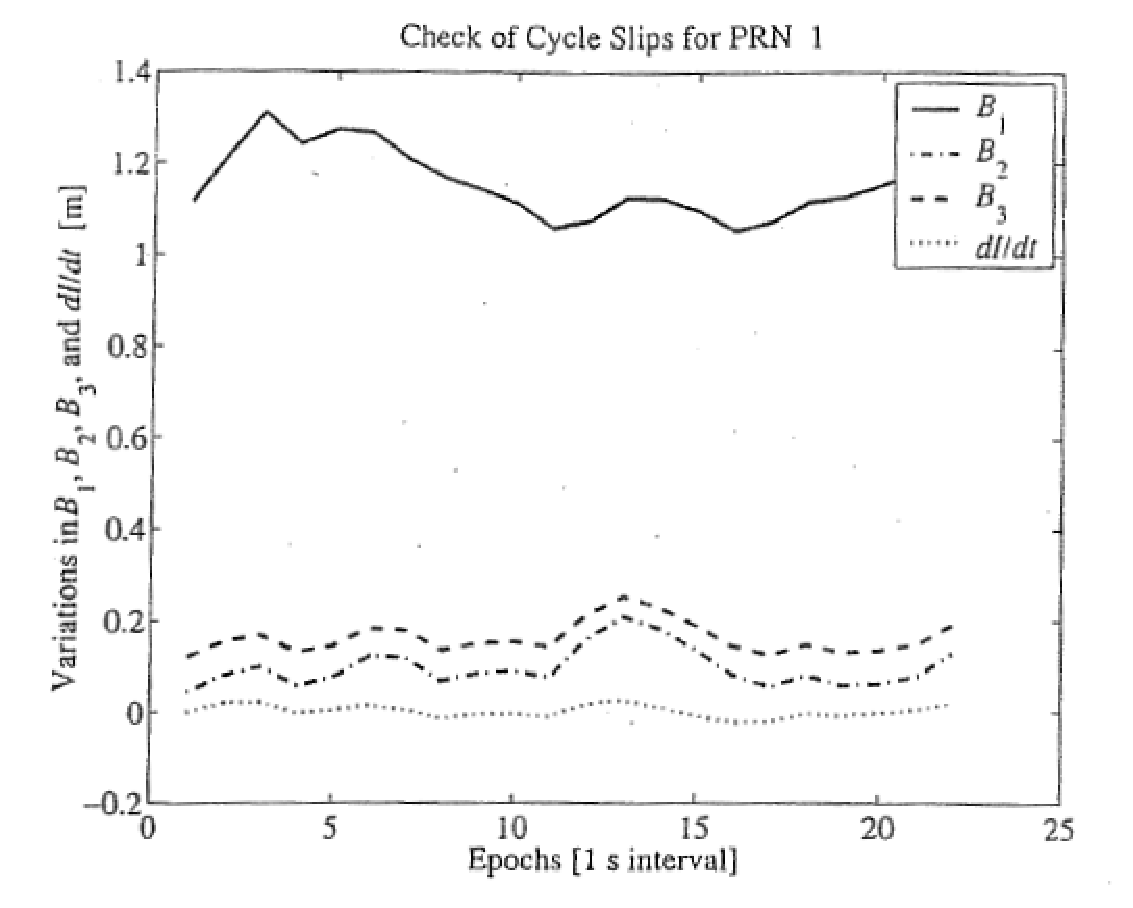
\includegraphics[width=0.4\linewidth]{TeX_files/Part03/chapter10/image/9-3}
	\caption{周跳探测}
	\label{fig:9-3}
\end{figure}

初步的数据验证可以利用站际单差。其目的是在卫星和接收机动态情况未知时,在GPS单差观测中探测周跳和异常值,以及钟的动态变化和大气层的影响。并且它仅利用单向观测值。对于这种所谓的完整性检测工作没有最少卫星数的要求。以下内容根据Kees de Jong (1998)提出的思想。

双频单差测量模式不能直接使用,因为此模式下的方程是奇异的。重新参数化将会使其可解。硬件延迟用$\eta$ 表示,每个历元k涉及到伪距R,包含的硬件延迟为:$R=\rho+cdt_{i}+T+I+\eta P_{1}$

\begin{equation}
	\begin{bmatrix}
		P_{1}\\
		P_{2}\\
		\Phi_{1}\\
		\Phi_{2}\\
	\end{bmatrix}
	=\begin{bmatrix}
		R\\
		R\\
		R\\
		R\\
	\end{bmatrix}_{k-1}
	+
	\begin{bmatrix}
		0\\
		\eta P_{2}-\eta P_{1}+(\alpha-1)I\\
		\eta \Phi_{1}-\eta P_{1}-2I+\lambda_{1}N_{1}\\
		\eta \Phi_{2}-\eta P_{1}+(-\alpha-1)I+\lambda_{2}N_{2}\\
	\end{bmatrix}_{k-1}
\end{equation}

$P_{1}$和$P_{2}$为伪距观测值,$\Phi_{1}$和$\Phi_{2}$为载波相位观测值,$N_{1}$和$N_{2}$为载波相位模糊度,$\lambda_{1}$和$\lambda_{2}$ 为波长:$\alpha=(f_{1}/f_{2})^{2}$

相关的频率是$f_{1}$和$f_{2}$, $\rho$ 是几何距离,I是电离层延迟(所有的项都是以米为单位的单差量)。

R可能不会随时间变化也很难利用低次多项式建模。但是上述矩阵利用方程2,3,4减去方程1可以消去R:
\begin{equation}
	\begin{bmatrix}
		P_{2}-P_{1}\\
		\Phi_{1}-P_{1}\\
		\Phi_{2}-P_{1}\\
	\end{bmatrix}_{k}
	=\begin{bmatrix}
		\alpha-1&0&0\\
		0&-2&0\\
		0&0&-\alpha-1\\
	\end{bmatrix}
	\begin{bmatrix}
		B_{1}\\
		B_{2}\\
		B_{3}\\
	\end{bmatrix}_{k}
\end{equation}

协方差矩阵包含“减法矩阵”和它的转置
$$
\Sigma_{differences}
=
\begin{bmatrix}
-1&1&0&0\\
-1&0&1&0\\
-1&0&0&1\\
\end{bmatrix}
\begin{bmatrix}
\sigma_{P_{1}}^{2}& & & \\
& \sigma_{P_{2}}^{2} & &\\
& &\sigma_{\Phi_{1}}^{2} & \\
& & & \sigma_{\Phi_{2}}^{2} \\
\end{bmatrix}
\begin{bmatrix}
-1&-1&-1\\
1&0&0\\
0&1&0\\
0&0&1\\
\end{bmatrix}_{k}
$$

参数 $B_{1}$, $B_{2}$和 $B_{3}$是与时间有关的电离层影响、常数项硬件延迟和载波模糊度的线性组合。

电离层影响将利用一阶多项式建模,即一个偏差值I和一个漂移值$\dot{I}$。动态模型(状态方程)为
$$
\begin{bmatrix}
I\\
\dot{I}\\
\end{bmatrix}_{k}
=\begin{bmatrix}
1&t_{k}-t_{k-1}\\
0&1\\
\end{bmatrix}
\begin{bmatrix}
I\\
\dot{I}\\
\end{bmatrix}_{k-1}
$$

在这种情况下$\dot{I}$=常数。则含有参数的动态模型变为如下形式:
$$
\begin{bmatrix}
B_{1}\\
B_{2}\\
B_{3}\\
\dot{I}\\
\end{bmatrix}_{k}
=\begin{bmatrix}
1&0&0&t_{k}-t_{k-1}\\
0&1&0&t_{k}-t_{k-1}\\
0&0&1&t_{k}-t_{k-1}\\
0&0&0&1\\
\end{bmatrix}
\begin{bmatrix}
B_{1}\\
B_{2}\\
B_{3}\\
\dot{I}\\
\end{bmatrix}_{k-1}
$$

同时测量模型变为
$$
\begin{bmatrix}
P_{2}-P_{1}\\
\Phi_{1}-P_{1}\\
\Phi_{2}-P_{1}\\
\end{bmatrix}_{k}
=\begin{bmatrix}
\alpha-1&0&0&0\\
0&-2&0&0\\
0&0&-\alpha-1&0\\
\end{bmatrix}
\begin{bmatrix}
B_{1}\\
B_{2}\\
B_{3}\\
\dot{I}\\
\end{bmatrix}_{k}
$$

仅利用以上模型,在载波观测值中探测周跳是可能的,甚至是当观测间隔$t_{k}-t_{k-1}$ 相对较大时,探测周跳也是可以实现的。

在实际探测中,载波L2上的跳动$|B_{2,k}-B_{2,k-1}|<\lambda_{1}$,载波L1上的跳动$|B_{3,k}-B_{3,k-1}|<\lambda_{2}$。若探测失败,则说明发生周跳并需要进行修复。